\documentclass[10pt,twocolumn]{article}

\usepackage[letterpaper,margin=0.72in,columnsep=0.25in]{geometry}
\usepackage{amsmath,amssymb}
\usepackage{booktabs,multirow,array}
\usepackage{graphicx}
\usepackage[dvipsnames]{xcolor}
\usepackage{microtype}
\usepackage{enumitem}
\usepackage{caption}
\usepackage{url}
\usepackage{hyperref}
\usepackage{tikz}
\usetikzlibrary{arrows.meta,positioning,fit,backgrounds,calc}

\hypersetup{
  colorlinks=true,
  linkcolor=MidnightBlue,
  citecolor=MidnightBlue,
  urlcolor=MidnightBlue,
  pdftitle={Zero-shot generative data assimilation for daily precipitation over Bangladesh},
  pdfauthor={Fahad Abdullah}
}

\setlength{\parindent}{1em}
\setlength{\parskip}{0pt}
\setlist{nosep,leftmargin=*}
\captionsetup{font=small,labelfont=bf}
\newcommand{\dd}{\,\mathrm{d}}
\newcommand{\mmday}{\mathrm{mm\,day^{-1}}}
\newcommand{\deggrid}[1]{#1$^\circ$}
\newcommand{\method}[1]{\textsc{#1}}
\newcolumntype{L}[1]{>{\raggedright\arraybackslash}p{#1}}
\newcommand{\placeholderfigure}[3]{%
  \par\medskip\noindent
  \begin{minipage}{\textwidth}
    \centering
    \fbox{\parbox[c][0.78in][c]{0.955\textwidth}{\centering
      \color{gray}\Large Figure #1 placeholder\\[0.35em]
      \normalsize #2}}
    \captionof{figure}{#3}
    \label{fig:#2}
  \end{minipage}\par\medskip
}

\title{Development and Process Validation of Zero-Shot Generative Data Assimilation\\
for 0.05$^\circ$ Daily Precipitation over Bangladesh}
\author{Fahad Abdullah\\
\small Affiliation to be added\\
\small Corresponding author information to be added}
\date{Draft generated \today}

\begin{document}
\maketitle

\begin{abstract}
Bangladesh needs spatially detailed daily precipitation fields, yet the available information is split among coarse gauge analyses, atmospheric reanalyses, satellite footprints, and a sparse national gauge network. We develop a probabilistic 0.05$^\circ$ ($\sim$5~km) framework that separates statistical downscaling from observation assimilation. A conditional rectified-flow U-Net is trained to generate CHIRPS-like fine-scale precipitation corrections from 0.5$^\circ$ CPC precipitation, five ERA5 state variables, static terrain, position, and season. At inference, the network is frozen and Bangladesh Meteorological Department (BMD) gauges and 0.1$^\circ$ IMERG footprints enter only through differentiable likelihood guidance. This separation allows observation networks and error models to change without retraining the prior.

We first evaluate the machinery in an observing-system simulation experiment (OSSE). With near-perfect pseudo-observations, withheld-station CRPS decreases from 6.94 to 1.12~$\mmday$ and sub-footprint correlation rises from 0.010 to 0.444, demonstrating recoverable fine-scale information. Realistic pseudo-observation errors give a smaller CRPS reduction, from 6.94 to 4.77~$\mmday$, and expose under-dispersion and excessive fine-scale member power. We then construct a real May 2018 experiment. Each BMD archive date is matched to 48 half-hourly IMERG V07B intervals spanning 03:00--03:00~UTC, and the complete CPC--ERA5 prior state is shifted back one calendar day because 21 of the 24 observation hours lie on that day. In a five-day, five-fold spatial holdout, gauge-only assimilation has the best pooled CRPS (4.638~$\mmday$), while simultaneous gauge--IMERG assimilation is close but worse (4.878~$\mmday$) and wins only one of five folds. We therefore select gauge-only provisionally, retire a sequential IMERG-to-gauge update, and treat the experiment as process validation rather than independent product validation because 2018 is inside the prior training period. The paper records the successful and failed ablations, the timing diagnosis, and the full-month and out-of-sample tests required before a Bangladesh rainfall product can be claimed.
\end{abstract}

\section{Introduction}

Daily rainfall over Bangladesh is controlled by monsoon flow, Bay of Bengal moisture transport, organized convection, and sharp orographic gradients near the Meghalaya Plateau and the Chittagong Hill Tracts. A coarse gridded product can represent the synoptic setting but cannot uniquely determine the location and texture of rainfall at 5~km. Conversely, a satellite product observes spatial organization at approximately 0.1$^\circ$ but contains retrieval, sampling, timing, and regime-dependent errors. National rain gauges provide direct point measurements but are too sparse to define a continuous field on their own.

The scientific problem is therefore not ordinary interpolation. It is to estimate a distribution over plausible 0.05$^\circ$ precipitation fields conditioned on a coarse atmospheric state and heterogeneous observations. A useful product should (i) improve independent gauge scores, (ii) retain realistic spatial variability rather than blur convective rainfall, (iii) quantify uncertainty, and (iv) remain modular when stations or satellite versions change.

We address this problem using a conditional generative prior and zero-shot data assimilation. The prior is a rectified-flow downscaler trained without BMD or IMERG. At inference, observations guide the frozen sampler through their physical operators and error models. The formulation follows the general idea of using generative models as non-Gaussian priors for inverse problems and data assimilation \cite{rozet2023,manshausen2025}, while replacing a diffusion trajectory with flow matching \cite{lipman2023,albergo2023}. The result is best understood as a development framework rather than a finished operational reanalysis. The evidence currently consists of a controlled OSSE and a bounded May 2018 real-data demonstration.

This manuscript makes four contributions. First, it defines a reproducible 0.5$^\circ$-to-0.05$^\circ$ probabilistic downscaling and posterior-sampling pipeline. Second, it establishes exact temporal and spatial observation operators for BMD and half-hourly IMERG. Third, it reports both successful and failed DA ablations, including dense satellite over-constraint, observation-error inflation, serial and simultaneous fusion, and background-date shifts. Fourth, it specifies a strict verification hierarchy in which withheld BMD gauges, not CHIRPS agreement or map sharpness, determine the selected real-data method.

\section{Data and study design}

\subsection{Domain and grids}

The production Bangladesh grid contains $128\times128$ cell centers at 0.05$^\circ$, spanning 87.6--94.0$^\circ$E and 20.3--26.7$^\circ$N. Training uses random $128\times128$ crops from a $256\times256$ WIDE grid spanning 84.0--96.8$^\circ$E and 16.0--28.8$^\circ$N. Latitudes are stored in ascending order. Training crops must contain at least 30\% valid land, avoiding nearly all-ocean targets.

\subsection{Gridded predictors and target}

Table~\ref{tab:data} summarizes the data streams. CHIRPS provides the 0.05$^\circ$ daily training target and is gauge-informed \cite{funk2015}. CPC Unified is a contemporaneous gauge analysis, not a forecast; its global 0.5$^\circ$ field is bilinearly mapped to the fine grid and paired with an explicit validity channel \cite{chen2008}. Missing CPC precipitation is represented as finite zero with validity equal to zero. ERA5 contributes total-column water vapor, CAPE, 10-m zonal and meridional wind, and mean sea-level pressure \cite{hersbach2020}. The operational CPC-conditioned checkpoint excludes ERA5 precipitation because CPC supplies the coarse precipitation base. Seven static fields comprise square-root-scaled elevation, standardized slope, the land mask, and four longitude/latitude positional encodings. Sine and cosine of day of year add seasonality.

The configured temporal split is 1981--2018 for training, 2019--2020 for validation, and 2021--2025 for testing. This split makes the May 2018 BMD experiment a workflow and assimilation test, not an independent temporal evaluation.

\begin{table*}[t]
\centering
\caption{Data streams and their roles. ``Prior'' means a model input available during training and inference; ``observation'' means the stream enters only the inference-time likelihood.}
\label{tab:data}
\small
\begin{tabular}{L{0.14\textwidth}L{0.11\textwidth}L{0.13\textwidth}L{0.14\textwidth}L{0.32\textwidth}}
\toprule
Stream & Native scale & Time support & Role & Processing used here \\
\midrule
CHIRPS v2 & 0.05$^\circ$, daily & 1981 onward & Prior training target; OSSE nature run & Selected onto the exact fine grid; contextual only in real-data verification because it is gauge-informed and trained the prior \cite{funk2015}. \\
CPC Unified & 0.5$^\circ$, daily & 1979 onward & Coarse precipitation prior & Bilinear remapping plus validity; transformed-space residual base \cite{chen2008}. \\
ERA5 & 0.25$^\circ$, hourly & 1940 onward & Atmospheric prior & Daily means of TCWV, CAPE, $u_{10}$, $v_{10}$, and MSLP; all fields move together in timing tests \cite{hersbach2020}. \\
IMERG Final V07B & 0.1$^\circ$, half-hourly & Satellite era & Dense observation & 48 rates accumulated to each BMD reporting day; exact $2\times2$ footprint operator; native random error propagated \cite{huffman2020}. \\
BMD gauges & Point, daily & Historical station archive & Sparse observation and primary validation & Legacy station-month matrix converted to a long daily table; spatially disjoint holdout folds. \\
Copernicus GLO-90 & $\sim$90 m, static & Static & Terrain prior & Area-aggregated to 0.05$^\circ$ before elevation and slope features. \\
\bottomrule
\end{tabular}
\end{table*}

\subsection{BMD observations}

The historical BMD archive is a station-month matrix with day-of-month columns and explicit missing markers. Station identifiers and coordinates are read from a separate catalog. Invalid calendar cells, negative values, values exceeding 1000~mm, and missing markers are removed; known spelling variants are reconciled explicitly. May 2018 contains 930 valid station-days from 30 stations, a 54.7\% wet-station-day fraction, and a maximum of 179~$\mmday$.

For the bounded experiment, a deterministic farthest-point algorithm creates geographically dispersed holdouts. The initial split assimilates 24 stations and withholds six. The stronger gate partitions all 30 stations into five disjoint spatial folds, so every station is withheld exactly once. The same station-days are used for every method being compared.

\subsection{Half-hourly IMERG and the BMD reporting day}

A BMD archive date $D$ is a 24-h accumulation ending at 03:00~UTC (09:00 Bangladesh Standard Time). The matching IMERG observation is therefore
\begin{equation}
 P_D^{\mathrm{IMERG}} = \sum_{k=1}^{48} r_k\,(0.5~\mathrm{h}),
 \label{eq:imergsum}
\end{equation}
where interval starts run from $D-1$ 03:00 through $D$ 02:30~UTC and $r_k$ is in mm~h$^{-1}$. The random-error depth is propagated as the square root of the sum of the 48 squared half-hourly error depths. All 48 unique intervals are mandatory; incomplete or duplicate windows fail preprocessing rather than being rescaled. May 1--31 requires 1,488 files, beginning 30 April at 03:00 and ending 31 May at 02:30. This operation already crosses the UTC date boundary; IMERG is not shifted backward by an additional day.

\section{Method}

\subsection{Conditional rectified-flow prior}

Let $x_1$ denote the standardized, transformed fine-grid precipitation correction and $x_0\sim\mathcal{N}(0,I)$. The linear probability path is
\begin{equation}
 x_t = t x_1 + (1-t)x_0, \qquad t\in(0,1).
 \label{eq:path}
\end{equation}
The U-Net $u_\theta(x_t,t,c)$ receives the noisy state, continuous time, and conditioning stack $c$, and is trained to regress the velocity $x_1-x_0$:
\begin{equation}
 \mathcal{L}_{\mathrm{FM}}=
 \mathbb{E}\left[\left\|M\odot\{u_\theta(x_t,t,c)-(x_1-x_0)\}\right\|_2^2\right],
 \label{eq:flowloss}
\end{equation}
where $M$ masks invalid ocean cells. Training samples $t$ from a logit-normal distribution. The transformed correction is defined relative to CPC,
\begin{equation}
 x_1 = \frac{T(P_{\mathrm{CHIRPS}})-T(P_{\mathrm{CPC}})-\mu_r}{\sigma_r},
 \label{eq:residual}
\end{equation}
so a zero physical correction reproduces CPC rather than climatology. Operational v1 uses $T(P)=\log(1+P/0.1)$, followed by training-only standardization.

The clean endpoint estimates used for guidance are
\begin{equation}
 \widehat{x}_1=x_t+(1-t)u_\theta,\qquad
 \widehat{x}_0=x_t-tu_\theta.
 \label{eq:endpoints}
\end{equation}
Heun integration transports independent noise draws toward an ensemble of fine-grid corrections. Reported OSSE plots used 30 steps; the current DA configuration uses 50 steps. We retain run metadata when reporting a result rather than silently replacing it with the latest configuration.

\subsection{Architecture and checkpoint provenance}

The operational checkpoint used by the reported OSSE and BMD experiments is \texttt{runs/prior\_h100\_cpc/best.pt}, referred to as CPC v1. The newest implemented configuration, CPC v2, is an architecture and training revision for future experiments. No result in this manuscript is attributed to v2 unless a checkpoint-embedded configuration establishes that provenance.

Both versions use an ADM-style U-Net with a 96-channel stem and multipliers $[1,2,3,4]$, giving resolutions/channels $128/96$, $64/192$, $32/288$, and $16/384$. Each encoder level has two residual blocks and the decoder has three after skip concatenation. Residual blocks use GroupNorm, SiLU, 3$\times$3 convolutions, dropout 0.2, and Fourier-time FiLM scale/shift. Self-attention is applied at 32 and 16 pixels and in the middle block with four heads. Downsampling uses a stride-2 3$\times$3 convolution; upsampling uses nearest-neighbor interpolation followed by a 3$\times$3 convolution. The v1 conditioning has 16 maps: seven dynamic, seven static, and two seasonal.

\begin{table*}[t]
\centering
\caption{Checkpoint used for reported results versus the latest implemented CPC v2 configuration. The separation prevents architectural improvements that have not yet been rerun from being credited with existing DA scores.}
\label{tab:architecture}
\small
\begin{tabular}{p{0.20\textwidth}p{0.35\textwidth}p{0.36\textwidth}}
\toprule
Component & CPC v1: reported-result checkpoint & CPC v2: latest implemented configuration \\
\midrule
Backbone & 96-channel ADM U-Net; multipliers 1/2/3/4; attention at 32 and 16; four heads; approximately 51.8M parameters from the source specification & Same core widths and attention; approximately 57.5M parameters from the source specification \\
Condition injection & All 16 condition maps concatenated at model input & Input concatenation plus learned condition pyramid injected at every U-Net scale through zero-initialized 1$\times$1 residual projections \\
Precipitation transform & Log1p for CPC and CHIRPS residual & Square root for CPC and CHIRPS residual \\
Objective & Masked flow-matching velocity loss & Flow loss plus 0.5$^\circ$ target coarse-consistency (weight 0.10) and CPC consistency (weight 0.02) \\
Sampling emphasis & Uniform daily sampling and random valid crops & 35\% top-decile wet-day mixture; 50\% chance of targeting a top-5\% wet pixel in a crop \\
Validation monitor & Sampled CRPS, EMA weights; reported best checkpoint near epoch 40 & Fifteen fixed July cases stratified over precipitation quantiles \\
Result status & Used in OSSE and real BMD--IMERG tables below & Implemented but not yet established as the source of reported results \\
\bottomrule
\end{tabular}
\end{table*}

The v1 model is trained for 150 epochs with AdamW, learning rate $1.5\times10^{-4}$, weight decay 0.01, 2,000 warmup steps followed by cosine decay, unit gradient clipping, batch size 32, and EMA decay 0.9995. Conditioning dropout is zero and classifier-free guidance is fixed to one, so the reported checkpoint is a conditional downscaler rather than a jointly trained unconditional model. Checkpoint selection uses sampled validation CRPS when available, not training flow loss alone.

\subsection{Zero-shot likelihood guidance}

Let $y$ stack observations and let $H$ map a candidate fine field to observation space. The desired posterior is
\begin{equation}
 p(x\mid y,c)\propto p_\theta(x\mid c)\,p(y\mid x).
 \label{eq:posterior}
\end{equation}
At trajectory time $t$, we evaluate a Gaussian likelihood around $H(\widehat{x}_1)$ with an early-time uncertainty term,
\begin{equation}
 \log p(y\mid x_t) = -\frac{1}{2}
 \left[y-H(\widehat{x}_1)\right]^\top V_t^{-1}
 \left[y-H(\widehat{x}_1)\right]+C,
 \label{eq:likelihood}
\end{equation}
\begin{equation}
 V_t=R+\Gamma\frac{(1-t)^2}{t^2}I.
 \label{eq:vt}
\end{equation}
The likelihood gradient is differentiated through the U-Net and observation operator, clipped for stability, and converted from a score correction to a velocity correction using the factor $(1-t)/t$. Observations therefore exert little influence when the trajectory is mostly noise and approach their specified error near the clean endpoint.

The active experiment has four matched arms: background, gauges only, IMERG only, and simultaneous gauges plus IMERG. Every ensemble member receives independently perturbed observations. IMERG perturbations are spatially correlated, while the simultaneous arm concatenates gauge and satellite likelihood terms in one guided trajectory. This is the operational meaning of ``simultaneous'' throughout the paper; it is not a two-stage analysis.

\subsection{Observation operators and error model}

The gauge operator converts a candidate from transformed model space to physical precipitation, bilinearly samples the 0.05$^\circ$ grid at each station, and returns to transformed observation space. The IMERG operator likewise acts in physical units and computes the exact mean of each nested $2\times2$ block of fine cells. Averaging in physical space is essential because precipitation transforms are nonlinear.

Gauge $R$ combines measurement and point-to-grid representativeness variance. IMERG uses the propagated native \texttt{randomError}, a transformed-space floor, and a representativeness term. To avoid treating thousands of correlated satellite pixels as independent, the controlled experiment retains every third 0.1$^\circ$ footprint in each direction. With correlation length $\ell=3$ coarse cells and stride $s=3$, the diagonal variance is multiplied by
\begin{equation}
 f_R=\max\left[1,2\pi(\ell/s)^2\right]=2\pi\approx6.28.
 \label{eq:rinflate}
\end{equation}
This retains 356 land footprints per day in the five-day experiment. It is an effective-sample approximation, not a claim that the residual covariance is truly diagonal. No fitted IMERG bias correction is used in the bounded results.

\subsection{Workflow}

Figure~\ref{fig:workflow} is the only populated figure in this draft. It separates offline prior learning, exact observation preparation, posterior sampling, and independent verification.

\begin{figure*}[t]
\centering
\resizebox{\textwidth}{!}{%
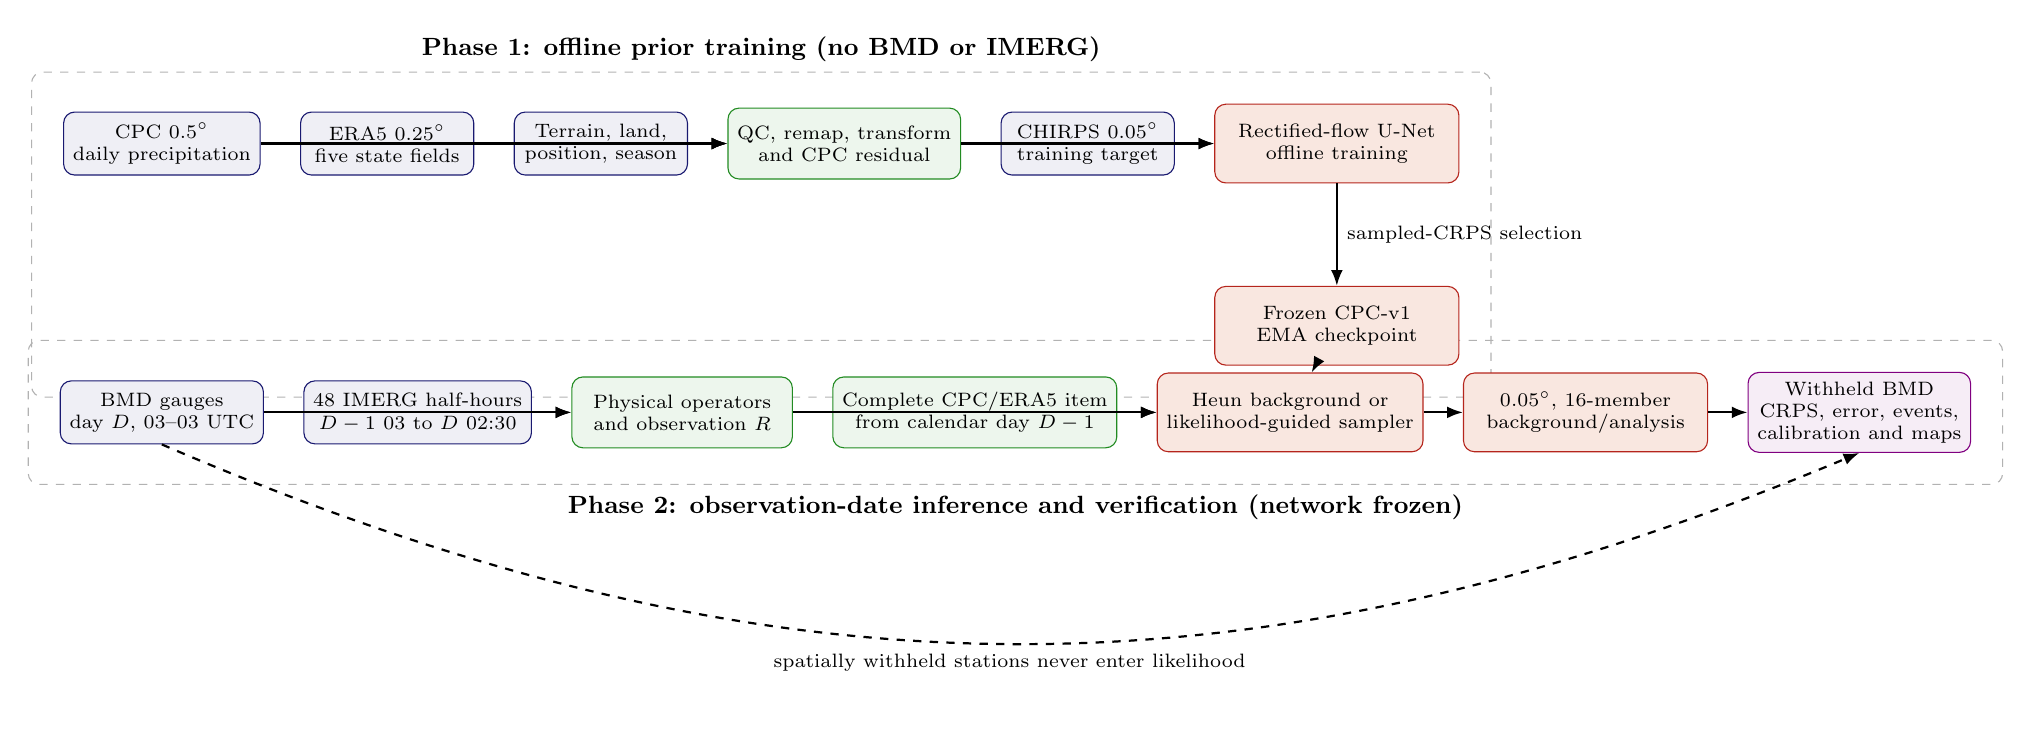
\begin{tikzpicture}[
  node distance=5mm and 5mm,
  every node/.style={font=\scriptsize,align=center},
  data/.style={draw=MidnightBlue,fill=MidnightBlue!7,rounded corners,minimum width=22mm,minimum height=8mm},
  proc/.style={draw=ForestGreen,fill=ForestGreen!8,rounded corners,minimum width=28mm,minimum height=9mm},
  model/.style={draw=BrickRed,fill=BrickRed!8,rounded corners,minimum width=31mm,minimum height=10mm},
  eval/.style={draw=Purple,fill=Purple!7,rounded corners,minimum width=27mm,minimum height=9mm},
  arr/.style={-{Latex[length=2mm]},thick},
  dashedarr/.style={-{Latex[length=2mm]},thick,dashed}
]
\node[data] (cpc) {CPC 0.5$^\circ$\\daily precipitation};
\node[data,right=of cpc] (era) {ERA5 0.25$^\circ$\\five state fields};
\node[data,right=of era] (static) {Terrain, land,\\position, season};
\node[proc,right=of static] (pack) {QC, remap, transform\\and CPC residual};
\node[data,right=of pack] (chirps) {CHIRPS 0.05$^\circ$\\training target};
\node[model,right=of chirps] (train) {Rectified-flow U-Net\\offline training};
\node[model,below=13mm of train] (frozen) {Frozen CPC-v1\\EMA checkpoint};

\draw[arr] (cpc) -- (pack);
\draw[arr] (era) -- (pack);
\draw[arr] (static) -- (pack);
\draw[arr] (pack) -- (train);
\draw[arr] (chirps) -- (train);
\draw[arr] (train) -- node[right]{sampled-CRPS selection} (frozen);

\node[data,below=26mm of cpc] (bmd) {BMD gauges\\day $D$, 03--03 UTC};
\node[data,right=of bmd] (imerg) {48 IMERG half-hours\\$D-1$ 03 to $D$ 02:30};
\node[proc,right=of imerg] (obs) {Physical operators\\and observation $R$};
\node[proc,right=of obs] (prioritem) {Complete CPC/ERA5 item\\from calendar day $D-1$};
\node[model,right=of prioritem] (sample) {Heun background or\\likelihood-guided sampler};
\node[model,right=of sample] (ensemble) {0.05$^\circ$, 16-member\\background/analysis};
\node[eval,right=of ensemble] (verify) {Withheld BMD\\CRPS, error, events,\\calibration and maps};

\draw[arr] (bmd) -- (obs);
\draw[arr] (imerg) -- (obs);
\draw[arr] (obs) -- (sample);
\draw[arr] (prioritem) -- (sample);
\draw[arr] (frozen) -- (sample);
\draw[arr] (sample) -- (ensemble);
\draw[arr] (ensemble) -- (verify);
\draw[dashedarr] (bmd.south) to[bend right=23] node[below]{spatially withheld stations never enter likelihood} (verify.south);

\begin{scope}[on background layer]
\node[draw=gray!60,dashed,rounded corners,fit=(cpc)(era)(static)(pack)(chirps)(train)(frozen),inner sep=4mm,label={[font=\small\bfseries]above:Phase 1: offline prior training (no BMD or IMERG)}] {};
\node[draw=gray!60,dashed,rounded corners,fit=(bmd)(imerg)(obs)(prioritem)(sample)(ensemble)(verify),inner sep=4mm,label={[font=\small\bfseries]below:Phase 2: observation-date inference and verification (network frozen)}] {};
\end{scope}
\end{tikzpicture}
}
\caption{End-to-end workflow. The prior learns a stochastic transformed-space correction from CPC and ERA5 to CHIRPS resolution. During inference, the network is frozen. A BMD archive day is paired with exactly 48 half-hourly IMERG intervals, while the complete CPC--ERA5 conditioning item is selected from the preceding calendar day. Gauge and satellite observations guide the same trajectory through a composite likelihood. Only stations excluded from that likelihood determine real-data method ranking.}
\label{fig:workflow}
\end{figure*}

\section{Experiments and verification}

\subsection{OSSE}

The OSSE treats independent held-out July CHIRPS fields as a 0.05$^\circ$ nature run. Exact $2\times2$ means form pseudo-IMERG footprints; a farthest-point design places 40 pseudo-stations, of which 20\% are withheld. Thirty days and 16 ensemble members are used. Background and analysis share random seeds so differences isolate assimilation.

Two observation regimes are considered. The near-perfect test retains only a small numerical error floor and tests whether the operators and guidance can reconstruct information across scales. The realistic test adds configured gauge and correlated satellite errors and is the more relevant stress test. The CHIRPS-on-CHIRPS construction remains optimistic because it omits actual satellite/gauge biases and product mismatch.

Verification includes fair ensemble CRPS, RMSE, bias, correlation, rank histograms, spread--skill, interval coverage, reliability, Brier score, CRPS by intensity, fractions skill score (FSS) \cite{roberts2008}, power spectra, normalized innovations, increment reach, and maps of changes in error and spread. Sub-footprint residual metrics test whether the analysis adds 0.05$^\circ$ information rather than merely reproducing a 0.1$^\circ$ mean.

\subsection{Real five-day process experiment}

The final bounded design uses May 1--5, 2018; exact half-hour IMERG windows; the $D-1$ complete CPC--ERA5 prior item; 16 members; four active arms; and five disjoint spatial folds. Across the folds, all 30 stations provide 150 withheld station-days. The timing offset is applied to CPC, CPC validity, all five ERA5 variables, the CPC residual base, and seasonal encoding together. BMD, IMERG, and observation-date CHIRPS context do not move.

The primary score is ensemble CRPS at withheld BMD stations \cite{gneiting2007}. Deterministic RMSE, MAE, bias, and correlation use the ensemble mean. We also report spread--skill, 90\% interval coverage, rank histograms, Brier scores and reliability at 1, 10, 25, and 50~$\mmday$, critical success index, day/station matrices, and collocated CPC, raw IMERG, CHIRPS, and inverse-distance-weighted gauge baselines. CHIRPS is explicitly excluded from method ranking because it is gauge-informed and trained the prior.

\section{Results}

\subsection{OSSE establishes capacity but exposes calibration failure}

Table~\ref{tab:osse} summarizes the remotely executed OSSE. Near-perfect observations reduce withheld CRPS by 83.9\%, full-field CRPS from 8.276 to 1.836~$\mmday$, and subgrid RMSE from 5.170 to 4.444~$\mmday$. Subgrid correlation rises from nearly zero to 0.444. These results demonstrate that the frozen prior and differentiable operators can reconstruct fine-scale degrees of freedom that are absent from a 0.1$^\circ$ footprint mean.

With realistic errors, withheld CRPS still improves by 31.2\%, but full-field improvement is only 9.6\%. The spread--skill ratio is 0.51 and rank-histogram deviation is 0.392; the ensemble is strongly under-dispersive. Member-to-truth fine-scale power ratio reaches 5.98, indicating excessive small-scale variability even though ensemble spread is too small relative to error. These are distinct failure modes: a member can be texturally noisy while the ensemble samples too narrow a set of storm locations or amplitudes. The realistic OSSE is therefore evidence of useful observational influence, not a calibrated reanalysis.

\begin{table*}[t]
\centering
\caption{OSSE results transcribed from remote run reports. CRPS values are in $\mmday$. ``Spread/skill'' below one indicates an ensemble that is too narrow relative to realized error.}
\label{tab:osse}
\small
\begin{tabular}{L{0.21\textwidth}L{0.11\textwidth}L{0.11\textwidth}L{0.23\textwidth}L{0.18\textwidth}}
\toprule
Metric & Realistic errors & Near-perfect errors & Interpretation & Gate \\
\midrule
Withheld CRPS, background $\rightarrow$ analysis & 6.94 $\rightarrow$ 4.77 & 6.94 $\rightarrow$ 1.12 & 31.2\% and 83.9\% improvements & Passes pointwise probabilistic skill \\
Full-field improvement & 9.6\% & 77.8\% & Realistic errors sharply reduce spatial benefit & Strong only for near-perfect case \\
Innovation standard deviation & 1.03 & 1.10 & Close to the unit-normalized target & Pass \\
Spread/skill & 0.51 & 0.59 & Both ensembles are under-dispersive & Fail \\
Rank-histogram deviation & 0.392 & 0.569 & Substantial non-uniformity & Fail \\
Land cells improved & 70.1\% & 89.5\% & Majority of cells improve & Pass as a spatial fraction \\
Subgrid RMSE, background $\rightarrow$ analysis & -- & 5.170 $\rightarrow$ 4.444 & Fine-scale residual becomes more accurate & Pass \\
Subgrid correlation, background $\rightarrow$ analysis & -- & 0.010 $\rightarrow$ 0.444 & Added information below footprint scale & Pass \\
Analysis 90\% coverage & -- & 0.807 & Better but below nominal 0.90 & Marginal \\
Fine-scale power, member/truth & 5.98 & 1.00 analysis (1.54 background) & Realistic members are too energetic at fine scales & Fail realistic; pass perfect \\
\bottomrule
\end{tabular}
\end{table*}

\subsection{Temporal alignment changes the real-data conclusion}

The first dense satellite experiment produced a catastrophic fused CRPS of 15.07~$\mmday$ versus 10.79 for the background and 4.74 for gauges only. Thinning footprints and inflating $R$ stabilized the likelihood but did not solve the mismatch. In the superseded calendar-day experiment, simultaneous CRPS was 6.587 and the serial IMERG-to-gauge result was 8.142, both worse than gauges alone at 4.742. Increasing total satellite $R$ inflation from 6.3 to 50.3 reduced simultaneous CRPS from 6.587 to 5.203, but it still did not beat gauges. This progression showed that simply weakening a misaligned satellite constraint tends toward the gauge-only solution rather than creating new skill.

Rebuilding the satellite accumulation from 240 half-hourly files for the five BMD windows changed the single-split results: IMERG-only CRPS improved from 10.16 to 6.28 and simultaneous CRPS from 6.59 to 4.27. A separate test then shifted the complete daily CPC--ERA5 prior item from $D$ to $D-1$, while leaving the exact BMD--IMERG window fixed. The single-split background CRPS improved from 10.79 to 6.19 and gauge-only from 4.74 to 4.04; simultaneous was 4.05, effectively tied with gauges.

The offset is physically plausible because a BMD day ending at 03:00~UTC contains 21 hours from calendar day $D-1$ and three hours from $D$. It is not an IMERG lag correction. A separate footprint-matched diagnostic found that same-date IMERG--CHIRPS correlation was best among lags of $\pm2$ days. The apparent spatial optimum was about one 0.1$^\circ$ cell east and north in the pooled five-day field, but its gain was below 0.05 and daily optima varied markedly. No fixed coordinate or satellite timestamp correction was applied.

\begin{table*}[t]
\centering
\caption{Development ablations for the real five-day experiment. Values are withheld-BMD CRPS in $\mmday$. Rows are not all directly comparable because ingestion and timing were corrected during development; the table records the decision sequence rather than presenting a single controlled factorial experiment.}
\label{tab:ablation}
\small
\setlength{\tabcolsep}{3pt}
\begin{tabular}{p{0.24\textwidth}ccccc p{0.20\textwidth}}
\toprule
Experiment & Background & Gauges & IMERG & Simultaneous & Sequential & Decision \\
\midrule
Uncontrolled dense fusion & 10.79 & 4.74 & -- & 15.07 & -- & Dense correlated likelihood rejected \\
Calendar-day, stride 3, $R\times6.3$ & 10.794 & 4.742 & 10.158 & 6.587 & 8.142 & Gauge-only wins; serial update poor \\
Calendar-day, $R\times12.6$ & 10.794 & 4.742 & 9.70 & 6.306 & -- & Satellite downweighted \\
Calendar-day, $R\times25.1$ & 10.794 & 4.742 & 9.89 & 5.853 & -- & Fusion approaches gauge solution \\
Calendar-day, $R\times50.3$ & 10.794 & 4.742 & 9.78 & 5.203 & -- & Still fails fusion gate \\
Exact 03--03 half-hour IMERG, offset 0 & 10.79 & 4.74 & 6.28 & 4.27 & 6.52 & Correct satellite window materially helps \\
Exact half-hour IMERG, prior offset $-1$ & 6.19 & 4.04 & 6.36 & 4.05 & 5.97 & Gauge and simultaneous tie on one split \\
\bottomrule
\end{tabular}
\end{table*}

\subsection{Rotated folds select gauges only provisionally}

The one-split fusion win does not survive spatial rotation. Table~\ref{tab:real} pools five disjoint folds, 30 stations, and 150 station-days under exact half-hour alignment and prior offset $-1$. Gauge-only has the lowest CRPS (4.638), RMSE (11.736), MAE (7.721), and bias magnitude (1.913). Simultaneous DA is close, with CRPS 4.878 and correlation 0.748, but its pooled CRPS penalty relative to gauges is 0.240~$\mmday$. It wins only fold 4, by 0.021~$\mmday$, whereas the predeclared gate requires lower pooled CRPS and at least three fold wins. Gauge-only is therefore the defensible current selection.

The calibration metrics require nuance. The fold-mean spread--skill ratios exceed one, which suggests over-dispersion in this small real-data sample, while gauge-only and simultaneous 90\% coverages are only 0.707 and 0.780. A single scalar spread--skill summary mixes intensity, stations, fold error, and observation error; it cannot guarantee calibrated quantiles. Rank, coverage, and intensity-stratified diagnostics remain necessary. This real-data behavior does not contradict OSSE under-dispersion because the truth, observation-error treatment, aggregation, and sample size differ.

\begin{table*}[t]
\centering
\caption{Exact-half-hour, background-offset-minus-one, five-fold real-data gate for May 1--5, 2018. All scores use BMD stations withheld from the likelihood. CRPS, RMSE, MAE, and bias are in $\mmday$. Correlation is Fisher pooled; spread--skill is the fold mean.}
\label{tab:real}
\small
\begin{tabular}{lrrrrrrr}
\toprule
Method & CRPS & RMSE & MAE & Bias & Correlation & Spread/skill & Cover90 \\
\midrule
Background & 6.149 & 14.995 & 11.801 & 7.922 & 0.675 & 1.556 & 0.933 \\
Gauges only & \textbf{4.638} & \textbf{11.736} & \textbf{7.721} & \textbf{1.913} & \textbf{0.748} & 1.337 & 0.707 \\
IMERG only & 6.280 & 15.264 & 11.236 & 7.674 & 0.718 & 1.684 & 0.853 \\
Simultaneous & 4.878 & 11.988 & 8.187 & 3.122 & 0.748 & 1.410 & 0.780 \\
\bottomrule
\end{tabular}
\end{table*}

\section{Development history and ablation decisions}

Several negative results materially changed the system.

\begin{enumerate}
\item \textbf{Absolute target to CPC residual.} Early absolute-target training could regress toward climatology and fail to beat the precipitation condition. The transformed residual makes an identity-like baseline explicit: zero correction reproduces CPC.
\item \textbf{Raw to nonlinear precipitation conditioning.} Log1p precipitation and square-root CAPE reduced domination by the heavy tail. CPC v2 now tests square-root target and base transforms as an explicit tail ablation.
\item \textbf{Classifier-free guidance rejected.} Earlier monitoring showed high-quantile spatial correlation decreasing as CFG increased above one. With v1 conditioning dropout set to zero, all reported sampling uses CFG equal to one.
\item \textbf{Background temperature separated from guided temperature.} Tempering an unguided prior can create positive physical bias after inverse transformation. The background therefore uses temperature one and no correctors; guided configurations may use 1.25 and corrector steps, but must be verified for dispersion and bias.
\item \textbf{EMA retained.} Non-EMA experiments produced noisier and less correlated sampled fields, so EMA weights are used for checkpoint selection and inference.
\item \textbf{Dense IMERG likelihood rejected.} Thousands of correlated pixels treated as independent overwhelmed the prior. Spatial thinning and effective correlation-area inflation were introduced.
\item \textbf{Sequential IMERG-to-gauge analysis retired.} A localized serial EnSRF with 75--150~km Gaspari--Cohn localization \cite{gaspari1999,whitaker2002} did not beat the direct simultaneous likelihood and was particularly poor on high-rain cases. The current comparison excludes it.
\item \textbf{CHIRPS-target real verification rejected.} Because CHIRPS trained the prior and incorporates gauges, map agreement with CHIRPS is descriptive context. Withheld BMD is the primary reference.
\item \textbf{Fixed IMERG spatial shift rejected.} Five-day lag/shift scans found no stable displacement. A coordinate correction requires a reproducible full-month gain, not visual alignment of one event.
\item \textbf{Latest v2 changes remain uncredited.} Multiscale conditioning, coarse consistency, wet sampling, and the square-root transform are implemented, but existing OSSE and BMD results remain CPC-v1 results until rerun.
\end{enumerate}

\section{Discussion}

\subsection{What the current evidence supports}

The near-perfect OSSE supports the central mechanism: a frozen conditional generative prior can use coarse footprints and gauges to recover 0.05$^\circ$ structure not directly observed at that scale. The realistic OSSE and real-data folds establish a stricter conclusion. Observation error, bias, representativeness, and timing dominate the practical problem. A sharper analysis or a closer fit at assimilated observations is insufficient; only independent withheld-station skill can justify fusion.

Gauge-only DA is currently the best-supported method for the bounded real test. Simultaneous assimilation remains scientifically plausible: it is close in pooled CRPS, has comparable correlation, and improves 90\% coverage relative to gauges. However, the satellite adds positive bias and does not pass the declared fold gate. The correct action is not to claim a fused product but to diagnose the satellite likelihood, fit bias correction outside the evaluation period, and retest over a larger independent sample.

The distinction between downscaling and forecasting is also important. CPC is a contemporaneous daily gauge analysis and ERA5 is a reanalysis. The current system estimates a high-resolution analysis for a completed day; it is not a lead-time precipitation forecast. A near-real-time product would require a latency-consistent background and IMERG Early/Late data with larger, separately validated error models.

\subsection{Limitations}

The real demonstration is only five days and 150 withheld station-days. More importantly, May 2018 lies inside the 1981--2018 prior training period. Although held-out gauges never enter the likelihood, temporal leakage through the learned CHIRPS target distribution prevents an independent product-skill claim. IMERG Final is gauge-adjusted and CHIRPS is gauge-informed, creating additional dependence. No fitted IMERG bias correction has yet been applied. The diagonal effective-$R$ treatment is only an approximation to dense correlated satellite error. Static daily conditioning cannot represent sub-daily storm evolution, and the sparse network limits verification of local extremes.

Uncertainty remains unresolved. The OSSE is under-dispersive, whereas the small real sample yields spread--skill values above one but under-nominal coverage for the best arms. The product cannot be called probabilistically calibrated until rank, coverage, reliability, and spread--skill behave consistently over longer, intensity-stratified, independently held-out periods.

\subsection{Required next experiments}

The immediate next gate is the already configured May 1--31 experiment: five disjoint station folds, 16 members, exact 03:00--03:00 IMERG windows, background offset $-1$, stride three, and $R$ inflation 6.28. All 30 stations should be withheld once, yielding up to 930 station-days. Paired uncertainty on score differences should use a circular multi-day block bootstrap rather than treating station-days as independent.

The subsequent scientific gate must retrain the prior with 2018 excluded, then repeat the same experiment without modifying hyperparameters. IMERG bias correction must be fitted on a disjoint period and evaluated at withheld BMD gauges. CPC v2 should then be compared with v1 using the same noise seeds and folds. Only after these tests should the selected method be extended to multiple monsoon and dry-season months, temporally held-out years, and alternative satellite latency products.

\section{Conclusion}

This work defines a modular generative-DA path to 0.05$^\circ$ daily precipitation over Bangladesh. Its strongest result is mechanistic: near-perfect OSSE observations recover sub-footprint structure and sharply improve withheld CRPS. Its most useful real-data result is cautionary: exact accumulation windows and checkpoint-day alignment matter as much as the assimilation algorithm, and a one-split fusion win disappears under rotated station withholding. Gauge-only assimilation is the provisional choice for the current five-day process test. A fused Bangladesh product is not yet scientifically justified; full-month, bias-corrected, and temporally independent evaluation is necessary.

\appendix
\section{Planned manuscript plots}

The workflow in Fig.~\ref{fig:workflow} is the only populated figure in this draft. The blank frames below define the remaining plot list and publication captions. They are deliberately left empty until the corresponding experiments pass their stated gates.

\onecolumn

\placeholderfigure{2}{data-domain}{Study domain, data support, and observation geometry. (a) Bangladesh and the WIDE training domain on a Cartopy Plate Carree map with national and first-order administrative boundaries; (b) native CPC, ERA5, IMERG, and 0.05$^\circ$ grid footprints; (c) BMD stations, five disjoint withheld folds, terrain, and land mask; and (d) temporal coverage and train/validation/test split.}

\placeholderfigure{3}{prior-learning}{Conditional-prior training and validation. Training flow-matching loss, EMA loss, sampled validation CRPS, ensemble-mean RMSE, spatial correlation, bias, spread, and 90\% coverage versus epoch. Vertical lines identify the sampled-CRPS checkpoint and the onset of overfitting; dotted baselines show CPC scored against CHIRPS on the identical cases.}

\placeholderfigure{4}{prior-cases}{Held-out downscaling cases for light, moderate, heavy, and extreme rainfall. Columns show CPC condition, CHIRPS target, ensemble mean, a representative member, ensemble-mean error, and ensemble spread. Each row shares a precipitation scale, and annotations report CRPS, RMSE, bias, correlation, and target intensity.}

\placeholderfigure{5}{osse-reconstruction}{OSSE design and multiscale reconstruction. Rows show representative withheld nature-run days; columns show 0.05$^\circ$ truth, 0.1$^\circ$ pseudo-satellite, background mean, analysis mean, an analysis member, background error, analysis error, and analysis spread. Assimilated and withheld pseudo-gauges are distinguished by filled and open markers.}

\placeholderfigure{6}{osse-verification}{OSSE probabilistic verification for realistic and near-perfect observation errors. Panels show withheld rank histograms, spread--skill, CRPS by rainfall intensity, reliability at 10 and 25~$\mmday$, empirical interval coverage, normalized innovations, and a metric matrix comparing background and analysis.}

\placeholderfigure{7}{osse-scale}{OSSE spatial-scale and impact diagnostics. Panels show FSS versus neighborhood width, isotropic power spectra for truth/mean/member, sub-footprint residual correlation and RMSE, mean error reduction, analysis increment magnitude, change in spread, benefit versus distance to the nearest assimilated station, and fraction of land cells improved by intensity.}

\placeholderfigure{8}{timing-alignment}{Temporal-alignment and geolocation diagnosis. Panels compare IMERG--CHIRPS pattern correlation over lags $-2$ to $+2$ days, same-day correlation over $\pm4$ native IMERG-cell shifts, daily optimum shifts, exact BMD reporting windows, and withheld-BMD score changes for CPC--ERA5 background offsets 0 and $-1$. No shift is adopted unless its gain is stable over the full month.}

\placeholderfigure{9}{five-day-products}{Direct station-collocated comparison for the bounded five-day experiment. CPC, raw IMERG, CHIRPS, gauge IDW, background, gauge-only DA, IMERG-only DA, and simultaneous DA are evaluated on exactly the same withheld BMD station-days. Panels show pooled deterministic metrics, absolute error by day and station, scatter about the 1:1 line, and rainfall-event contingency scores.}

\placeholderfigure{10}{rotated-fold-gate}{Five-fold spatial method gate for exact-half-hour IMERG and background offset $-1$. Panels show CRPS by fold, simultaneous-minus-gauge CRPS, pooled CRPS with fold variability, deterministic metrics, empirical 90\% coverage by fold, and Brier scores at 1, 10, 25, and 50~$\mmday$.}

\placeholderfigure{11}{real-spatial-cases}{Representative real-observation DA cases. Columns show CPC input, BMD-aligned IMERG, CHIRPS context, background mean, gauge-only mean, IMERG-only mean, simultaneous mean, analysis-minus-background, and analysis spread. Map panels use Cartopy and mark assimilated versus withheld BMD stations; CHIRPS is labelled non-independent context, not truth.}

\placeholderfigure{12}{full-month-primary}{Full-May primary verification against rotated withheld BMD gauges. Panels show method CRPS with paired block-bootstrap intervals, CRPS by day and station, deterministic metric matrix, station-space scatter, CRPSS relative to background, and the spatial distribution of station-level added value. This figure determines the selected real-data method.}

\placeholderfigure{13}{full-month-calibration}{Full-May ensemble calibration and event performance. Panels show rank histograms, spread--skill by intensity, empirical 50/80/90\% interval coverage, reliability diagrams, Brier skill, CSI/POD/FAR, and CRPS for 0--1, 1--5, 5--10, 10--25, 25--50, and $>50~\mmday$. Bootstrap intervals use paired multi-day blocks.}

\placeholderfigure{14}{full-month-spatial}{Full-May spatial behavior without claiming an independent gridded truth. Panels show mean background and analysis, mean absolute increment, change in ensemble spread, increment reach from gauges, wet-day frequency, fine-scale departure from 0.2$^\circ$ means, power spectra, and Cartopy station maps of withheld-BMD error change.}

\placeholderfigure{15}{ablation-summary}{Ablation synthesis using matched folds and seeds. Panels compare CPC v1 and v2, log1p and square-root transforms, absolute and residual targets, multiscale conditioning, EMA, sampler temperature/correctors, IMERG stride and $R$ inflation, bias correction, gauges/IMERG/simultaneous likelihoods, and ensemble sizes. Only independently evaluated settings are ranked; historical ingestion experiments are visually separated from controlled ablations.}

\section{Reproducibility checklist}

\begin{center}
\centering
\captionof{table}{Current evidence status. A check means the implementation and result are available; ``configured'' means code exists but the experiment is not yet a manuscript result.}
\label{tab:status}
\small
\begin{tabular}{p{0.34\textwidth}p{0.15\textwidth}p{0.42\textwidth}}
\toprule
Item & Status & Evidence boundary \\
\midrule
CPC-v1 prior and sampled-CRPS checkpoint & Complete & Used for all reported OSSE and BMD results; checkpoint metadata should be archived with final submission. \\
Near-perfect and realistic OSSE & Complete & Remote logs available; final archive should include JSON outputs and exact sampler metadata. \\
Exact BMD 03--03 UTC IMERG preparation & Complete & Five days use 240 half-hourly files; all footprints passed QC. \\
Five-day, five-fold spatial holdout & Complete & 150 station-days; gauges only selected provisionally. \\
Full May, five-fold holdout & Configured & No skill values may be reported until pooled outputs and block-bootstrap intervals exist. \\
CPC-v2 prior & Implemented & Latest architecture, but not the source of current results. \\
IMERG bias correction & Planned & Must be fitted outside the evaluation period. \\
Temporally independent 2018 evaluation & Planned & Requires retraining with 2018 excluded. \\
\bottomrule
\end{tabular}
\end{center}

\clearpage
\twocolumn

\begin{thebibliography}{99}

\bibitem{albergo2023}
M. S. Albergo, N. M. Boffi, and E. Vanden-Eijnden.
Stochastic interpolants: A unifying framework for flows and diffusions.
\emph{arXiv:2303.08797}, 2023.

\bibitem{chen2008}
M. Chen, W. Shi, P. Xie, V. B. S. Silva, V. E. Kousky, R. W. Higgins, and J. E. Janowiak.
Assessing objective techniques for gauge-based analyses of global daily precipitation.
\emph{Journal of Geophysical Research: Atmospheres}, 113:D04110, 2008.

\bibitem{funk2015}
C. Funk et al.
The climate hazards infrared precipitation with stations---a new environmental record for monitoring extremes.
\emph{Scientific Data}, 2:150066, 2015.
doi:10.1038/sdata.2015.66.

\bibitem{gaspari1999}
G. Gaspari and S. E. Cohn.
Construction of correlation functions in two and three dimensions.
\emph{Quarterly Journal of the Royal Meteorological Society}, 125:723--757, 1999.
doi:10.1002/qj.49712555417.

\bibitem{gneiting2007}
T. Gneiting and A. E. Raftery.
Strictly proper scoring rules, prediction, and estimation.
\emph{Journal of the American Statistical Association}, 102:359--378, 2007.

\bibitem{hersbach2020}
H. Hersbach et al.
The ERA5 global reanalysis.
\emph{Quarterly Journal of the Royal Meteorological Society}, 146:1999--2049, 2020.
doi:10.1002/qj.3803.

\bibitem{huffman2020}
G. J. Huffman, D. T. Bolvin, E. J. Nelkin, and coauthors.
Integrated Multi-satellite Retrievals for the Global Precipitation Measurement (GPM) Mission (IMERG).
In V. Levizzani et al., editors, \emph{Satellite Precipitation Measurement}, Springer, 2020.
doi:10.1007/978-3-030-24568-9\_19.

\bibitem{lipman2023}
Y. Lipman, R. T. Q. Chen, H. Ben-Hamu, M. Nickel, and M. Le.
Flow matching for generative modeling.
In \emph{International Conference on Learning Representations}, 2023.
arXiv:2210.02747.

\bibitem{manshausen2025}
P. Manshausen et al.
Generative data assimilation of sparse weather station observations at kilometer scales.
\emph{Journal of Advances in Modeling Earth Systems}, 17:e2024MS004505, 2025.
doi:10.1029/2024MS004505.

\bibitem{roberts2008}
N. M. Roberts and H. W. Lean.
Scale-selective verification of rainfall accumulations from high-resolution forecasts of convective events.
\emph{Monthly Weather Review}, 136:78--97, 2008.
doi:10.1175/2007MWR2123.1.

\bibitem{rozet2023}
F. Rozet and G. Louppe.
Score-based data assimilation for a two-layer quasi-geostrophic model.
\emph{arXiv:2310.01853}, 2023.

\bibitem{whitaker2002}
J. S. Whitaker and T. M. Hamill.
Ensemble data assimilation without perturbed observations.
\emph{Monthly Weather Review}, 130:1913--1924, 2002.

\end{thebibliography}

\end{document}
